\documentclass[%
 mph,%
 reprint,%
]{revtex4-2}

\usepackage{titlesec}
% Format section headings with sans-serif font
\titleformat{\section}
{\large\bfseries\sffamily}
{\thesection}{1em}{}
% Format subsection headings with sans-serif font
\titleformat{\subsection}
{\bfseries\sffamily}
{\thesubsection}{1em}{}

% Format subsubsection headings with sans-serif font
\titleformat{\subsubsection}
{\bfseries\sffamily}
{\thesubsubsection}{1em}{}
\usepackage{mathtools, amssymb}
\usepackage{xcolor}
\usepackage{newcomputermodern}
\usepackage{hyperref}
\hypersetup{
    colorlinks = true,
    linkcolor={red!50!black},
    citecolor={blue!50!black},
    urlcolor={blue!80!black}
}
\def\mpl{M_{\rm\sss Pl}}
\def\sbh{S_{\rm\sss BH}}
\def\shr{S_{\rm\sss HR}}
\def\rout{\rho_{\rm out}}
\def\rin{\rho_{\rm in}}
\def\op{\omega_+}
\def\om{\omega_-}
\def\p{\varphi}
\begin{document}


\title[PHY644 TermPaper (Spring Semester 2023)]{Entropy and Area}
\thanks{PHY644 TermPaper (Spring Semester 2023)}

\author{Aditya Dev (MS19022) }
 \email{ms19022@iisermohali.ac.in}
\affiliation{Department of Physical Science, Indian Institute of Science Education and Research Mohali}%



\date{15 April, 2023}% It is always \today, today,
             %  but any date may be explicitly specified

\begin{abstract}
\centering
\textit{Journal Paper Details:} \vspace{5pt}\\ 
\textbf{Title:} Entropy and Area \\
\textbf{Author:} \href{https://web.physics.ucsb.edu/~mark/}{Mark Srednicki} \\
\textbf{Journal:} Physical Review Letters 71 (5), 666-669 (1993)\\
\textbf{DOI:}  \href{https://journals.aps.org/prl/abstract/10.1103/PhysRevLett.71.666}{10.1103/PhysRevLett.71.666}
\end{abstract}

\maketitle
\tableofcontents
\section{Introduction}
In this above paper, author explores the relationship between entropy and the area of a black hole's event horizon in the context of quantum mechanics. The ground state density matrix for massless free field is traced over the degree of freedom inside a imaginary sphere, and the resulting entropy of this (\textit{i.e the partially traced})  system is found to be directly proportional to the surface area of the enclosing sphere (Ref~\onlinecite{srednicki}). This work has had a significant impact on the study of black holes and the relationship between thermodynamics and quantum mechanics and derives the now-famous black hole entropy formula.

\section{Black Hole Entropy Formula}
The study of black hole thermodynamics began in the 1970's, when Stephen Hawking showed that black holes emit radiation due to quantum effects\cite{Hawking:1975vcx}. This discovery suggested that black holes have a temperature and can be described using thermodynamic  entropy. However, it was unclear how to relate a black hole's entropy to its physical properties.

This paper builds on the work of Jacob Bekenstein \cite{PhysRevD.7.2333}, who proposed in the 1970s that the entropy of a black hole is proportional to its surface area. Author takes this idea one step further by showing that the entropy of a black hole can be derived from the quantum states of its constituent particles.

The key result is the derivation of the black hole entropy formula, which relates the entropy  to the area of black hole event horizon. The formula is given by:
\begin{equation}
S = \kappa M^2 A
\end{equation}
where $S$ is the entropy  $A = 4\pi R^2$ is the area of its event horizon, and where \(\kappa 
\) is a constant whose numerical value depends on definition of \(M\). This formula is same as for the intrinsic entropy of black hole
\begin{equation}
    S_{BH} = \frac{1}{4} M_{pl} A
\end{equation}
where \(M_{pl}\) is the Planck mass. 
It suggests that the laws of thermodynamics, which describe the behavior of macroscopic systems, may also apply to black holes, often described as the most extreme objects in the universe.


\section{Quantum States and Entropy of a Black Hole}
We begin by considering the quantum states of a black hole. and assume that a black hole is made up of a large number of particles, each with its own quantum state (\emph{we will model the particles using N harmonic oscillators}). The total number of possible quantum states is given by the following equation:
\begin{equation}
N = e^{S/k_B}
\end{equation}
where $N$ is the number of quantum states, $S$ is the entropy of the black hole, and $k_B$ is Boltzmann's constant.


To establish the formula for entropy we take a simple model; a system described by two coupled harmonic oscillators. The Hamiltonian of the system is given as:
\begin{equation}
    H = \frac{1}{2}\left[p_1^2 + p_2^2 + k_0(x_1^2 + x_2^2)
                               + k_1(x_1-x_2)^2\right]
\end{equation}
The normalized ground state solution is:
\begin{equation}
    \psi_0(x_1,x_2)=\pi^{-1/2}(\op\om)^{1/4}
                   e^{-(\op x_+^2 + \om x_-^2)/2}
\end{equation}

where \(x_\pm=(x_1\pm x_2)/\sqrt2\), \(\op=k_0^{1/2}\),
and \(\om=(k_0+2k_1)^{1/2}\).
We first trace over the ``inside'' oscillator, resulting in a density matrix for the ``outside'' degree of freedom:
\begin{equation}
    \begin{gathered}
    \rout(x_2,x'_2) = \int_{-\infty}^{+\infty} dx_1\,\psi_0(x_1,x_2)
                                                \psi^*_0(x_1,x'_2) \\
        = \pi^{-1/2}(\gamma-\beta)^{1/2}
       \exp\left[-\gamma(x_2^2+x^{\prime 2}_2)/2+\beta x_2x'_2\right]
    \end{gathered}
\end{equation}
where $\beta=\frac14(\op-\om)^2/(\op+\om)$ and
$\gamma-\beta=2\op\om/(\op+\om)$.
To find the eigenvalues $p_n$ of $\rout(x,x')$, we notice:
\begin{equation}
    \label{eq:eigen_value_equation}
    \int_{-\infty}^{+\infty}dx'\,\rout(x,x')f_n(x')=p_n f_n(x)
\end{equation}
Also, we know that the entropy formula is given as:
\begin{equation}
    S=-\sum_n p_n\log p_n
\end{equation}

The solution to Eq.~\ref{eq:eigen_value_equation} is given as:
\begin{equation}
\label{eq:eigenvalues}
    \begin{gathered}
        p_n = (1-\xi)\xi^n\\
        f_n(x) = H_n(\alpha^{1/2}x)\exp(-\alpha x^2/2)
    \end{gathered}
\end{equation}
where $H_n$ is a Hermite polynomial,
$\alpha=(\gamma^2-\beta^2)^{1/2}=(\op\om)^{1/2}$,
$\xi=\beta/(\gamma+\alpha)$, and $n$ runs from zero to infinity.
Eq.~\ref{eq:eigenvalues} implies that $\rout$ is equivalent to a thermal density matrix for a single harmonic oscillator specified by frequency $\alpha$ and temperature $T=\alpha/\log(1/\xi)$.  The corresponding entropy is
\begin{equation}
    S(\xi)=-\log(1-\xi)-\frac{\xi}{1 - \xi}\log\xi
\end{equation}
where $\xi$ is a function only of  $k_1/k_0$.

The above formula we derived for a coupled oscillator can be generalized to \(N\) particle, for details one can Ref~(\onlinecite{srednicki}). The final relation is:
\begin{equation}
    S_l(n,N)=\xi_l(n)\left[-\log\xi_l(n)+1\right]
\end{equation}
where \(N\) is number of harmonic oscillators and \(n\) are sites over which the ground state density matrix is traced. Also, \begin{equation}
    \xi_l(n)=\frac{n(n+1)(2n+1)^2}{64 l^2 (l+1)^2}+O(l^{-6})
\end{equation}

\begin{figure}[!ht]
    \centering
    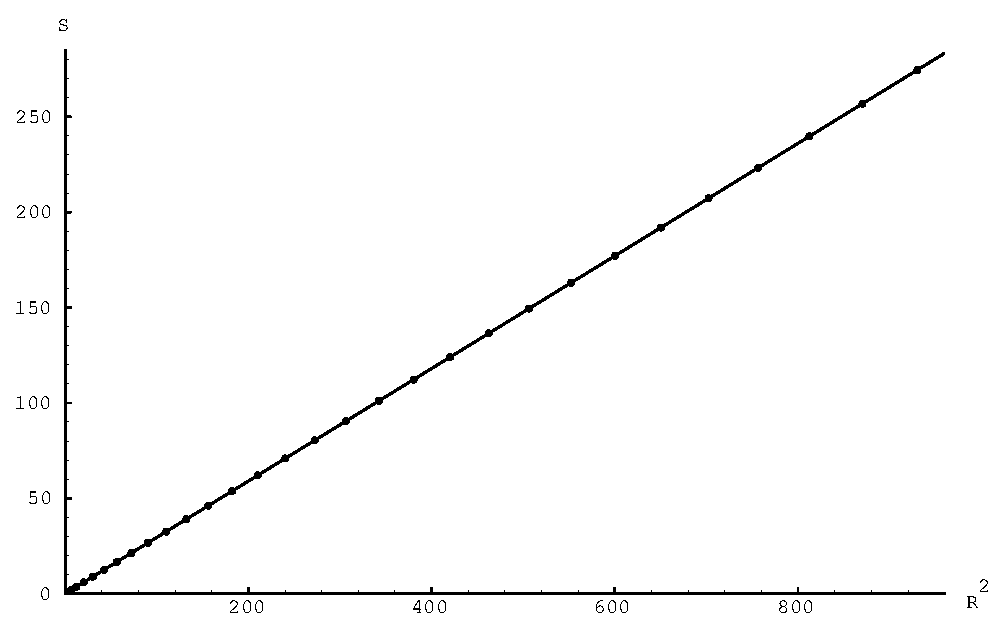
\includegraphics[scale=0.5]{msfig.eps}
    \caption{The entropy after tracing the ground state scalar field over the dof inside a sphere of radius}
    \label{fig:my_label}
\end{figure}
We define $R=(n+ \frac{1}{2})a$, a radius midway between the outermost point which was traced over, and the innermost point which was not.  The \textit{numerically} computed values of $S(n,N)$  shown for $N=60$ and $1\le n\le 30$ as a function
of $R^2$ in Fig~\ref{fig:my_label}.  The points are fit by 
\begin{equation}
    S=0.30 M^2 R^2  = 0.30 M^2 \frac{A}{4\pi}
\end{equation}


This formula shows that the entropy of a black hole is proportional to its surface area, as Bekenstein\cite{PhysRevD.7.2333} had proposed. However, Srednicki's derivation provides a quantum mechanical explanation for this relationship.


\section{Comments and Conclusion}
The Mark Srednicki's ``Entropy and Area" introduced the black hole entropy formula, which relates the entropy of a black hole to the area of its event horizon. This formula is significant because it suggests that black holes have thermodynamic properties and establishes a connection between thermodynamics and gravity. The validity of the black hole entropy formula has been confirmed through various calculations and thought experiments, including Stephen Hawking's famous ``black hole thought experiment,"\cite{Hawking:1975vcx} which demonstrated that black holes emit thermal radiation. Srednicki's paper has contributed significantly to the field of black hole physics, and has inspired further research into the relationship between thermodynamics and gravity, including the holographic principle. This principle suggests that the information content of a black hole can be encoded on its event horizon.

\bibliography{reference}
\end{document}
